\documentclass{standalone}
\usepackage{tikz}
\usetikzlibrary{patterns, positioning}


\begin{document}
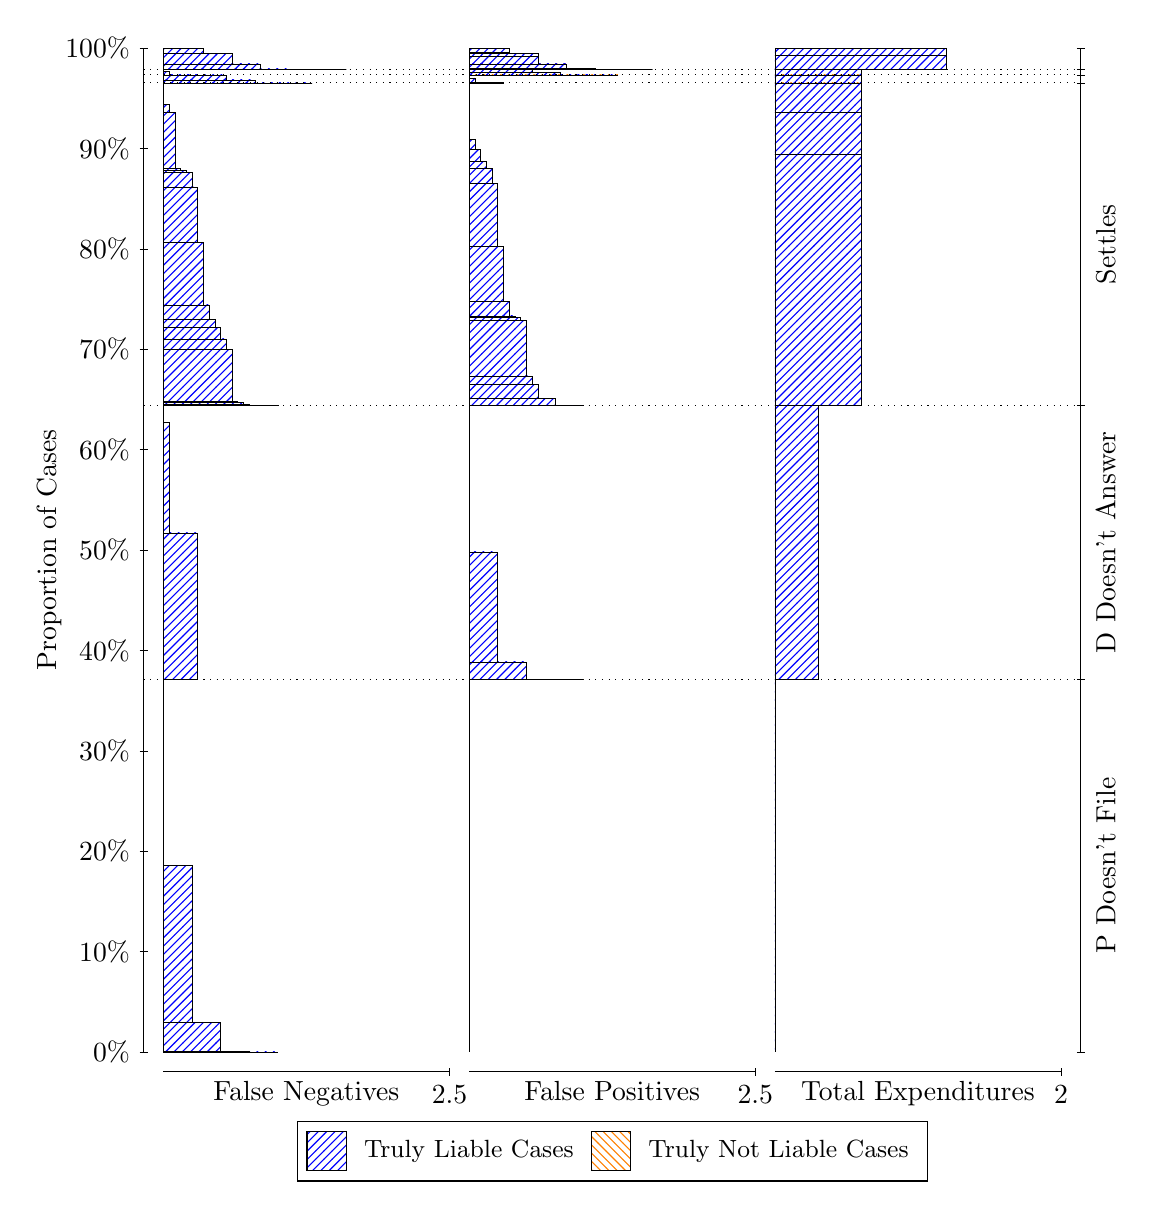
\begin{tikzpicture}
\draw[black, very thin] (1.5,1.75) -- (1.5,14.5);
\node[rotate=90, text=black, anchor=center] at (0.3, 8.125) {Proportion of Cases};
\draw[black, very thin] (1.45,1.75) -- (1.55,1.75);
\node[text=black, anchor=east] at (1.45, 1.75) {0\%};
\draw[black, very thin] (1.45,3.025) -- (1.55,3.025);
\node[text=black, anchor=east] at (1.45, 3.025) {10\%};
\draw[black, very thin] (1.45,4.3) -- (1.55,4.3);
\node[text=black, anchor=east] at (1.45, 4.3) {20\%};
\draw[black, very thin] (1.45,5.575) -- (1.55,5.575);
\node[text=black, anchor=east] at (1.45, 5.575) {30\%};
\draw[black, very thin] (1.45,6.85) -- (1.55,6.85);
\node[text=black, anchor=east] at (1.45, 6.85) {40\%};
\draw[black, very thin] (1.45,8.125) -- (1.55,8.125);
\node[text=black, anchor=east] at (1.45, 8.125) {50\%};
\draw[black, very thin] (1.45,9.4) -- (1.55,9.4);
\node[text=black, anchor=east] at (1.45, 9.4) {60\%};
\draw[black, very thin] (1.45,10.675) -- (1.55,10.675);
\node[text=black, anchor=east] at (1.45, 10.675) {70\%};
\draw[black, very thin] (1.45,11.95) -- (1.55,11.95);
\node[text=black, anchor=east] at (1.45, 11.95) {80\%};
\draw[black, very thin] (1.45,13.225) -- (1.55,13.225);
\node[text=black, anchor=east] at (1.45, 13.225) {90\%};
\draw[black, very thin] (1.45,14.5) -- (1.55,14.5);
\node[text=black, anchor=east] at (1.45, 14.5) {100\%};

\draw[black, very thin] (13.4,1.75) -- (13.4,14.5);
\draw[black, very thin] (13.35,1.75) -- (13.45,1.75);
\node[anchor=west] at (13.35, 1.75) {};
\draw[black, very thin] (13.35,6.4846) -- (13.45,6.4846);
\node[anchor=west] at (13.35, 6.4846) {};
\draw[black, very thin] (13.35,9.9604) -- (13.45,9.9604);
\node[anchor=west] at (13.35, 9.9604) {};
\draw[black, very thin] (13.35,14.057) -- (13.45,14.057);
\node[anchor=west] at (13.35, 14.057) {};
\draw[black, very thin] (13.35,14.159) -- (13.45,14.159);
\node[anchor=west] at (13.35, 14.159) {};
\draw[black, very thin] (13.35,14.232) -- (13.45,14.232);
\node[anchor=west] at (13.35, 14.232) {};
\draw[black, very thin] (13.35,14.5) -- (13.45,14.5);
\node[anchor=west] at (13.35, 14.5) {};

\draw[black, very thin, pattern color=blue, pattern=north east lines] (1.75,1.75) rectangle (3.2033,1.75);
\draw[black, very thin, pattern color=blue, pattern=north east lines] (1.75,1.75) rectangle (2.84,1.7532);
\draw[black, very thin, pattern color=blue, pattern=north east lines] (1.75,1.7532) rectangle (2.4767,2.1289);
\draw[black, very thin, pattern color=blue, pattern=north east lines] (1.75,2.1289) rectangle (2.1133,4.1206);
\draw[black, very thin, pattern color=orange, pattern=north west lines] (1.75,4.1206) rectangle (1.75,4.1206);
\draw[black, very thin, pattern color=blue, pattern=north east lines] (1.75,4.1206) rectangle (1.75,6.4846);
\draw[black, very thin, pattern color=blue, pattern=north east lines] (1.75,6.4846) rectangle (2.186,8.3434);
\draw[black, very thin, pattern color=blue, pattern=north east lines] (1.75,8.3434) rectangle (1.8227,9.7408);
\draw[black, very thin, pattern color=orange, pattern=north west lines] (1.75,9.7408) rectangle (1.75,9.7408);
\draw[black, very thin, pattern color=blue, pattern=north east lines] (1.75,9.7408) rectangle (1.75,9.9604);
\draw[black, very thin, pattern color=blue, pattern=north east lines] (1.75,9.9604) rectangle (3.2033,9.9605);
\draw[black, very thin, pattern color=blue, pattern=north east lines] (1.75,9.9605) rectangle (3.058,9.9605);
\draw[black, very thin, pattern color=blue, pattern=north east lines] (1.75,9.9605) rectangle (2.9127,9.9608);
\draw[black, very thin, pattern color=blue, pattern=north east lines] (1.75,9.9608) rectangle (2.84,9.9784);
\draw[black, very thin, pattern color=blue, pattern=north east lines] (1.75,9.9784) rectangle (2.7673,10.001);
\draw[black, very thin, pattern color=blue, pattern=north east lines] (1.75,10.001) rectangle (2.6947,10.01);
\draw[black, very thin, pattern color=blue, pattern=north east lines] (1.75,10.01) rectangle (2.622,10.676);
\draw[black, very thin, pattern color=blue, pattern=north east lines] (1.75,10.676) rectangle (2.5493,10.807);
\draw[black, very thin, pattern color=blue, pattern=north east lines] (1.75,10.807) rectangle (2.4767,10.957);
\draw[black, very thin, pattern color=blue, pattern=north east lines] (1.75,10.957) rectangle (2.404,11.05);
\draw[black, very thin, pattern color=blue, pattern=north east lines] (1.75,11.05) rectangle (2.3313,11.239);
\draw[black, very thin, pattern color=blue, pattern=north east lines] (1.75,11.239) rectangle (2.2587,12.035);
\draw[black, very thin, pattern color=blue, pattern=north east lines] (1.75,12.035) rectangle (2.186,12.736);
\draw[black, very thin, pattern color=blue, pattern=north east lines] (1.75,12.736) rectangle (2.1133,12.92);
\draw[black, very thin, pattern color=blue, pattern=north east lines] (1.75,12.92) rectangle (2.0407,12.942);
\draw[black, very thin, pattern color=blue, pattern=north east lines] (1.75,12.942) rectangle (1.968,12.976);
\draw[black, very thin, pattern color=blue, pattern=north east lines] (1.75,12.976) rectangle (1.8953,13.681);
\draw[black, very thin, pattern color=blue, pattern=north east lines] (1.75,13.681) rectangle (1.8227,13.786);
\draw[black, very thin, pattern color=orange, pattern=north west lines] (1.75,13.786) rectangle (1.75,13.786);
\draw[black, very thin, pattern color=blue, pattern=north east lines] (1.75,13.786) rectangle (1.75,14.057);
\draw[black, very thin, pattern color=blue, pattern=north east lines] (1.75,14.057) rectangle (3.6393,14.057);
\draw[black, very thin, pattern color=blue, pattern=north east lines] (1.75,14.057) rectangle (3.276,14.057);
\draw[black, very thin, pattern color=blue, pattern=north east lines] (1.75,14.057) rectangle (2.9127,14.095);
\draw[black, very thin, pattern color=blue, pattern=north east lines] (1.75,14.095) rectangle (2.5493,14.158);
\draw[black, very thin, pattern color=blue, pattern=north east lines] (1.75,14.158) rectangle (2.186,14.159);
\draw[black, very thin, pattern color=orange, pattern=north west lines] (1.75,14.159) rectangle (1.75,14.159);
\draw[black, very thin, pattern color=blue, pattern=north east lines] (1.75,14.159) rectangle (2.186,14.16);
\draw[black, very thin, pattern color=blue, pattern=north east lines] (1.75,14.16) rectangle (1.8227,14.205);
\draw[black, very thin, pattern color=orange, pattern=north west lines] (1.75,14.205) rectangle (1.75,14.205);
\draw[black, very thin, pattern color=blue, pattern=north east lines] (1.75,14.205) rectangle (1.75,14.232);
\draw[black, very thin, pattern color=blue, pattern=north east lines] (1.75,14.232) rectangle (4.0753,14.232);
\draw[black, very thin, pattern color=blue, pattern=north east lines] (1.75,14.232) rectangle (3.712,14.232);
\draw[black, very thin, pattern color=blue, pattern=north east lines] (1.75,14.232) rectangle (3.3487,14.236);
\draw[black, very thin, pattern color=blue, pattern=north east lines] (1.75,14.236) rectangle (2.9853,14.298);
\draw[black, very thin, pattern color=blue, pattern=north east lines] (1.75,14.298) rectangle (2.622,14.433);
\draw[black, very thin, pattern color=blue, pattern=north east lines] (1.75,14.433) rectangle (2.2587,14.495);
\draw[black, very thin, pattern color=blue, pattern=north east lines] (1.75,14.495) rectangle (1.8953,14.5);
\draw[black, very thin, pattern color=orange, pattern=north west lines] (1.75,14.5) rectangle (1.75,14.5);
\draw[black, very thin, pattern color=blue, pattern=north east lines] (1.75,14.5) rectangle (1.75,14.5);
\draw[black, very thin, pattern color=orange, pattern=north west lines] (5.6333,1.75) rectangle (5.6333,1.75);
\draw[black, very thin, pattern color=blue, pattern=north east lines] (5.6333,1.75) rectangle (5.6333,6.4846);
\draw[black, very thin, pattern color=orange, pattern=north west lines] (5.6333,6.4846) rectangle (7.0867,6.4846);
\draw[black, very thin, pattern color=blue, pattern=north east lines] (5.6333,6.4846) rectangle (7.0867,6.4846);
\draw[black, very thin, pattern color=blue, pattern=north east lines] (5.6333,6.4846) rectangle (6.7233,6.4852);
\draw[black, very thin, pattern color=blue, pattern=north east lines] (5.6333,6.4852) rectangle (6.36,6.7042);
\draw[black, very thin, pattern color=blue, pattern=north east lines] (5.6333,6.7042) rectangle (5.9967,8.1017);
\draw[black, very thin, pattern color=blue, pattern=north east lines] (5.6333,8.1017) rectangle (5.6333,9.9604);
\draw[black, very thin, pattern color=orange, pattern=north west lines] (5.6333,9.9604) rectangle (7.0867,9.9604);
\draw[black, very thin, pattern color=blue, pattern=north east lines] (5.6333,9.9604) rectangle (7.0867,9.9606);
\draw[black, very thin, pattern color=orange, pattern=north west lines] (5.6333,9.9606) rectangle (6.9413,9.9606);
\draw[black, very thin, pattern color=blue, pattern=north east lines] (5.6333,9.9606) rectangle (6.9413,9.9606);
\draw[black, very thin, pattern color=orange, pattern=north west lines] (5.6333,9.9606) rectangle (6.796,9.9606);
\draw[black, very thin, pattern color=blue, pattern=north east lines] (5.6333,9.9606) rectangle (6.796,9.9608);
\draw[black, very thin, pattern color=blue, pattern=north east lines] (5.6333,9.9608) rectangle (6.7233,10.049);
\draw[black, very thin, pattern color=orange, pattern=north west lines] (5.6333,10.049) rectangle (6.6507,10.049);
\draw[black, very thin, pattern color=blue, pattern=north east lines] (5.6333,10.049) rectangle (6.6507,10.049);
\draw[black, very thin, pattern color=blue, pattern=north east lines] (5.6333,10.049) rectangle (6.578,10.049);
\draw[black, very thin, pattern color=orange, pattern=north west lines] (5.6333,10.049) rectangle (6.5053,10.049);
\draw[black, very thin, pattern color=blue, pattern=north east lines] (5.6333,10.049) rectangle (6.5053,10.231);
\draw[black, very thin, pattern color=blue, pattern=north east lines] (5.6333,10.231) rectangle (6.4327,10.336);
\draw[black, very thin, pattern color=blue, pattern=north east lines] (5.6333,10.336) rectangle (6.36,11.042);
\draw[black, very thin, pattern color=blue, pattern=north east lines] (5.6333,11.042) rectangle (6.2873,11.075);
\draw[black, very thin, pattern color=blue, pattern=north east lines] (5.6333,11.075) rectangle (6.2147,11.098);
\draw[black, very thin, pattern color=blue, pattern=north east lines] (5.6333,11.098) rectangle (6.142,11.281);
\draw[black, very thin, pattern color=blue, pattern=north east lines] (5.6333,11.281) rectangle (6.0693,11.983);
\draw[black, very thin, pattern color=blue, pattern=north east lines] (5.6333,11.983) rectangle (5.9967,12.778);
\draw[black, very thin, pattern color=blue, pattern=north east lines] (5.6333,12.778) rectangle (5.924,12.968);
\draw[black, very thin, pattern color=blue, pattern=north east lines] (5.6333,12.968) rectangle (5.8513,13.061);
\draw[black, very thin, pattern color=blue, pattern=north east lines] (5.6333,13.061) rectangle (5.7787,13.211);
\draw[black, very thin, pattern color=blue, pattern=north east lines] (5.6333,13.211) rectangle (5.706,13.342);
\draw[black, very thin, pattern color=blue, pattern=north east lines] (5.6333,13.342) rectangle (5.6333,14.057);
\draw[black, very thin, pattern color=orange, pattern=north west lines] (5.6333,14.057) rectangle (6.0693,14.057);
\draw[black, very thin, pattern color=blue, pattern=north east lines] (5.6333,14.057) rectangle (6.0693,14.059);
\draw[black, very thin, pattern color=blue, pattern=north east lines] (5.6333,14.059) rectangle (5.706,14.121);
\draw[black, very thin, pattern color=blue, pattern=north east lines] (5.6333,14.121) rectangle (5.6333,14.159);
\draw[black, very thin, pattern color=orange, pattern=north west lines] (5.6333,14.159) rectangle (7.5227,14.159);
\draw[black, very thin, pattern color=blue, pattern=north east lines] (5.6333,14.159) rectangle (7.5227,14.159);
\draw[black, very thin, pattern color=blue, pattern=north east lines] (5.6333,14.159) rectangle (7.1593,14.159);
\draw[black, very thin, pattern color=blue, pattern=north east lines] (5.6333,14.159) rectangle (6.796,14.187);
\draw[black, very thin, pattern color=blue, pattern=north east lines] (5.6333,14.187) rectangle (6.4327,14.231);
\draw[black, very thin, pattern color=blue, pattern=north east lines] (5.6333,14.231) rectangle (6.0693,14.232);
\draw[black, very thin, pattern color=orange, pattern=north west lines] (5.6333,14.232) rectangle (7.9587,14.232);
\draw[black, very thin, pattern color=blue, pattern=north east lines] (5.6333,14.232) rectangle (7.9587,14.232);
\draw[black, very thin, pattern color=orange, pattern=north west lines] (5.6333,14.232) rectangle (7.5953,14.232);
\draw[black, very thin, pattern color=blue, pattern=north east lines] (5.6333,14.232) rectangle (7.5953,14.232);
\draw[black, very thin, pattern color=orange, pattern=north west lines] (5.6333,14.232) rectangle (7.232,14.232);
\draw[black, very thin, pattern color=blue, pattern=north east lines] (5.6333,14.232) rectangle (7.232,14.237);
\draw[black, very thin, pattern color=blue, pattern=north east lines] (5.6333,14.237) rectangle (6.8687,14.298);
\draw[black, very thin, pattern color=orange, pattern=north west lines] (5.6333,14.298) rectangle (6.8687,14.298);
\draw[black, very thin, pattern color=blue, pattern=north east lines] (5.6333,14.298) rectangle (6.8687,14.299);
\draw[black, very thin, pattern color=blue, pattern=north east lines] (5.6333,14.299) rectangle (6.5053,14.389);
\draw[black, very thin, pattern color=orange, pattern=north west lines] (5.6333,14.389) rectangle (6.5053,14.389);
\draw[black, very thin, pattern color=blue, pattern=north east lines] (5.6333,14.389) rectangle (6.5053,14.434);
\draw[black, very thin, pattern color=blue, pattern=north east lines] (5.6333,14.434) rectangle (6.142,14.448);
\draw[black, very thin, pattern color=blue, pattern=north east lines] (5.6333,14.448) rectangle (6.142,14.496);
\draw[black, very thin, pattern color=blue, pattern=north east lines] (5.6333,14.496) rectangle (5.7787,14.496);
\draw[black, very thin, pattern color=blue, pattern=north east lines] (5.6333,14.496) rectangle (5.7787,14.5);
\draw[black, very thin, pattern color=blue, pattern=north east lines] (5.6333,14.5) rectangle (5.6333,14.5);
\draw[black, very thin, pattern color=orange, pattern=north west lines] (9.5167,1.75) rectangle (9.5167,1.75);
\draw[black, very thin, pattern color=blue, pattern=north east lines] (9.5167,1.75) rectangle (9.5167,6.4846);
\draw[black, very thin, pattern color=orange, pattern=north west lines] (9.5167,6.4846) rectangle (10.062,6.4846);
\draw[black, very thin, pattern color=blue, pattern=north east lines] (9.5167,6.4846) rectangle (10.062,9.9604);
\draw[black, very thin, pattern color=orange, pattern=north west lines] (9.5167,9.9604) rectangle (10.607,9.9604);
\draw[black, very thin, pattern color=blue, pattern=north east lines] (9.5167,9.9604) rectangle (10.607,13.154);
\draw[black, very thin, pattern color=orange, pattern=north west lines] (9.5167,13.154) rectangle (10.607,13.154);
\draw[black, very thin, pattern color=blue, pattern=north east lines] (9.5167,13.154) rectangle (10.607,13.687);
\draw[black, very thin, pattern color=orange, pattern=north west lines] (9.5167,13.687) rectangle (10.607,13.687);
\draw[black, very thin, pattern color=blue, pattern=north east lines] (9.5167,13.687) rectangle (10.607,14.057);
\draw[black, very thin, pattern color=orange, pattern=north west lines] (9.5167,14.057) rectangle (10.607,14.057);
\draw[black, very thin, pattern color=blue, pattern=north east lines] (9.5167,14.057) rectangle (10.607,14.159);
\draw[black, very thin, pattern color=orange, pattern=north west lines] (9.5167,14.159) rectangle (10.607,14.159);
\draw[black, very thin, pattern color=blue, pattern=north east lines] (9.5167,14.159) rectangle (10.607,14.232);
\draw[black, very thin, pattern color=orange, pattern=north west lines] (9.5167,14.232) rectangle (11.697,14.232);
\draw[black, very thin, pattern color=blue, pattern=north east lines] (9.5167,14.232) rectangle (11.697,14.403);
\draw[black, very thin, pattern color=orange, pattern=north west lines] (9.5167,14.403) rectangle (11.697,14.403);
\draw[black, very thin, pattern color=blue, pattern=north east lines] (9.5167,14.403) rectangle (11.697,14.5);
\draw[black, dotted] (1.5,6.4846) -- (13.4,6.4846);
\draw[black, dotted] (1.5,9.9604) -- (13.4,9.9604);
\draw[black, dotted] (1.5,14.057) -- (13.4,14.057);
\draw[black, dotted] (1.5,14.159) -- (13.4,14.159);
\draw[black, dotted] (1.5,14.232) -- (13.4,14.232);
\draw[black, very thin] (1.75,1.5) -- (5.3833,1.5);
\node[text=black, anchor=north] at (3.5667, 1.5) {False Negatives};
\draw[black, very thin] (5.3833,1.45) -- (5.3833,1.55);
\node[text=black, anchor=north] at (5.3833, 1.45) {2.5};

\draw[black, very thin] (5.6333,1.5) -- (9.2667,1.5);
\node[text=black, anchor=north] at (7.45, 1.5) {False Positives};
\draw[black, very thin] (9.2667,1.45) -- (9.2667,1.55);
\node[text=black, anchor=north] at (9.2667, 1.45) {2.5};

\draw[black, very thin] (9.5167,1.5) -- (13.15,1.5);
\node[text=black, anchor=north] at (11.333, 1.5) {Total Expenditures};
\draw[black, very thin] (13.15,1.45) -- (13.15,1.55);
\node[text=black, anchor=north] at (13.15, 1.45) {2};

\node[text=black, centered, rotate=90] at (13.72, 4.1173) {P Doesn't File};
\node[text=black, centered, rotate=90] at (13.72, 8.2225) {D Doesn't Answer};
\node[text=black, centered, rotate=90] at (13.72, 12.009) {Settles};




\draw (7.449999999999999,1.5) node[draw=none] (baseCoordinate) {};
\begin{scope}[align=center]
        \matrix[scale=0.5, draw=black, below=0.5cm of baseCoordinate, nodes={draw}, column sep=0.1cm]{
            \node[rectangle, draw, minimum width=0.5cm, minimum height=0.5cm, pattern color=blue, pattern=north east lines] {}; &
            \node[draw=none, font=\small, text=black] (B) {Truly Liable Cases}; &
            \node[rectangle, draw, minimum width=0.5cm, minimum height=0.5cm, pattern color=orange, pattern=north west lines] {}; &
            \node[draw=none, font=\small, text=black] (B) {Truly Not Liable Cases}; \\
            };
\end{scope}

\end{tikzpicture}
\end{document}